\section{Validación y métricas de evaluación}
\label{sec:diseno}
\subsection{Comparaciones del sprint}
Se mantienen dos contrastes separados: A--D modifica las features con Ridge fijo; la comparación de cinco algoritmos conserva la geometría A. Ambos reutilizan casos y particiones. No se realizó una búsqueda de hiperparámetros ni un cruce completo de todos los algoritmos con todas las representaciones. Por tanto, la mejora de los momentos con Ridge no se atribuye al bosque aleatorio.

Las variantes son acumulativas: B--A añade momentos, C--B añade la razón y D--C retira un bloque. El control auxiliar de media predice el promedio del entrenamiento; A es el baseline geométrico. La regla registrada exige reducir MAE al menos 5\%, mejorar en al menos 60\% de grupos, no aumentar RMSE y no aumentar MAE al reservar familias. Son criterios del proyecto, no tolerancias mecánicas ni pruebas de significancia. Una mejora primaria insuficiente se mantiene en evaluación; un deterioro incremental se descarta.

\subsection{Estrategia de validación}
El protocolo principal aplica \textit{LeaveOneGroupOut} (LOGO) a la combinación $(n_Y,h_f,h_p)$ \cite{sklearnlogo}. Sus 24 particiones reservan una configuración completa cada vez: 22 grupos contienen un caso y dos contienen dos. Los entrenamientos incluyen 25 o 24 casos, respectivamente. Los pares nominales se mantienen juntos para evitar que una misma combinación aparezca simultáneamente a ambos lados de la partición. La geometría reservada puede compartir familia con el entrenamiento; por tanto, esta evaluación no demuestra transferencia a otra arquitectura completa.

El protocolo secundario reserva sucesivamente $Y=4$, $Y=5$ y $Y=6$. Evalúa ocho, nueve y nueve casos, con 18, 17 y 17 casos de entrenamiento. Cada observación recibe una predicción fuera de muestra (OOF) por protocolo y variante. Las listas de casos son idénticas para A--D y están guardadas en \ruta{particiones.json}. LOGO no usa barajado; la semilla 42 identifica la configuración general, pero ni el particionado ni Ridge con SVD dependen de ella. No existe un holdout final independiente.

En cada fold se ajusta el siguiente flujo con los casos de entrenamiento:
\begin{center}\small
Contrato de entradas $\to$ imputación $\to$ representación A--D\\
$\to$ filtro de constantes $\to$ estandarización $\to$ Ridge.
\end{center}
La evaluación solo transforma y predice con los parámetros ya ajustados \cite{sklearnleakage}. El registro de auditoría conserva índices, medianas, columnas, medias y escalas para verificar esa separación. El agrupamiento trata una dependencia conocida, pero no certifica independencia física donde faltan identificadores de lote o espécimen.

\subsection{Métricas}
Sea $e_i=y_i-\widehat y_i$ el residuo OOF de cada caso evaluado. Las métricas se calculan concatenando las predicciones reservadas:
\begin{align}
\mathrm{MAE}&=\frac{1}{n}\sum_{i=1}^{n}|e_i|,&
\mathrm{RMSE}&=\sqrt{\frac{1}{n}\sum_{i=1}^{n}e_i^2},\\
\mathrm{MedAE}&=\operatorname{mediana}_i(|e_i|),&
R^2_{\mathrm{OOF}}&=1-\frac{\sum_i e_i^2}{\sum_i(y_i-\overline y)^2}.
\end{align}
MAE, RMSE y MedAE se expresan en newtons. MAE es el error absoluto promedio; RMSE penaliza más los errores grandes y MedAE describe el error absoluto central. $R^2$ compara la suma de errores con la variabilidad global observada y puede ser negativo. No representa un porcentaje de aciertos. No se calcula ni promedia $R^2$ en folds unitarios.

Para el contraste $V-R$, $\Delta\mathrm{MAE}=\mathrm{MAE}_V-\mathrm{MAE}_R$; un valor negativo favorece la variante. La reducción porcentual es $100(\mathrm{MAE}_R-\mathrm{MAE}_V)/\mathrm{MAE}_R$. La desviación estándar muestral de MAE entre folds describe heterogeneidad, no un error estándar independiente, pues los entrenamientos se solapan. MAE OOF pondera casos; la media y desviación de MAE por fold ponderan grupos. El tiempo registrado suma ajuste y predicción de los folds.

\section{Resultados del Feature Engineering}
\label{sec:resultados}
\subsection{Resultados del baseline}
A obtuvo MAE de 13,247~N, RMSE de 16,346~N, MedAE de 11,941~N y $R^2_{\mathrm{OOF}}=0{,}923$. El control de media alcanzó MAE de 56,309~N. La geometría aporta capacidad predictiva bajo reserva de configuraciones, aunque la separación entre familias contribuye al buen valor agregado de $R^2$. Este resultado no garantiza el mismo error para una familia excluida: el MAE de A aumenta a 57,637~N en ese protocolo y su $R^2$ resulta negativo (Tabla~\ref{tab:familias}).

\subsection{Variante 1: momentos de sección}
B mantuvo las dimensiones originales y añadió dos funciones geométricas de la sección. El MAE bajó a 12,835~N: 0,412~N o 3,11\% menos que A. RMSE disminuyó 0,143~N, hasta 16,203~N; MedAE fue 11,780~N y $R^2=0{,}924$. El tiempo registrado aumentó de 0,290 a 0,683~s. La mejora es pequeña respecto de la dispersión de errores y no acredita un mecanismo de rotura por flexión.

B mejoró el error medio en 15 de 24 grupos (62,5\%), pero no alcanzó el umbral de reducción del 5\%. El MAE al reservar familias aumentó 0,016~N, de 57,637 a 57,654~N. La regla de adopción, aplicada literalmente, conserva B en evaluación. La diferencia secundaria es mínima; su importancia aquí es que no aporta evidencia de transferencia favorable, no que demuestre un deterioro significativo.

\subsection{Variante 2 y reducción posterior}
C añadió $L_{p/f}$ a los momentos. Su MAE fue 12,914~N, 0,079~N mayor que B (+0,62\%), acompañado de RMSE de 16,327~N. Aunque C sigue 2,51\% por debajo de A, no mejora su referencia inmediata B. La asociación global de la razón con el objetivo no se traduce en beneficio incremental. Se descarta esta adición para el conjunto propuesto, sin afirmar que carezca de utilidad en otros modelos o campañas.

D retiró el bloque de tres columnas directas y produjo MAE de 17,035~N y RMSE de 21,136~N. Frente a C, el MAE creció 4,121~N (+31,91\%); frente a A, 3,788~N (+28,60\%). La representación reducida conservó nueve predictores efectivos, como A, pero con un contenido funcional distinto. La parsimonia nominal no compensó el cambio de parametrización. Este resultado rechaza la retirada conjunta bajo el protocolo evaluado; no estima la importancia individual de cada columna eliminada.

\subsection{Tabla comparativa principal}
La decisión de C y D utiliza su referencia incremental, mientras que la columna $\Delta$ permite comparar todos los conjuntos con A.
\begin{table}[htbp]
\centering\small\setstretch{1.0}
\caption{Resultados OOF por configuración nominal. Errores y dispersión en N; tiempo en segundos.}
\label{tab:principal}
\setlength{\tabcolsep}{3.2pt}
\begin{tabular}{@{}crrrrrrrl@{}}
\toprule
Exp. & Features & MAE & RMSE & $R^2$ & $\Delta$ vs. A & $s_{\mathrm{CV}}$ & Tiempo & Decisión \\
\midrule
\tableinput tablas/principal.tex
\bottomrule
\end{tabular}
\par\smallskip\footnotesize Fuente: \ruta{comparacion_experimentos.csv}. $s_{\mathrm{CV}}$: desviación estándar del MAE de los 24 folds, no intervalo de confianza. Decisiones sujetas a la regla de la sección~\ref{sec:diseno}.
\end{table}
\begin{table}[htbp]
\centering\small\setstretch{1.0}
\caption{Comprobación secundaria: predicciones OOF al reservar familias completas.}
\label{tab:familias}
\begin{tabular}{@{}lrrrr@{}}
\toprule
Experimento & MAE (N) & RMSE (N) & MedAE (N) & $R^2_{\mathrm{OOF}}$ \\
\midrule
\tableinput tablas/familias.tex
\bottomrule
\end{tabular}
\par\smallskip\footnotesize Fuente: mismo registro, protocolo \texttt{familia}; tres folds. Cada caso se evalúa una vez. No son resultados de entrenamiento.
\end{table}

\subsection{Comparación visual principal}
La Figura~\ref{fig:mae} muestra la ventaja limitada de B y el deterioro de D, junto con el cambio de escala del error al excluir familias. Las barras no llevan intervalos inferenciales: se dispone de una evaluación interna dependiente, no de campañas independientes repetidas. En el protocolo secundario todos los $R^2$ son negativos; aun así, los MAE son menores que el del control de media del entrenamiento (80,593~N). Son referencias distintas y no deben confundirse.
\begin{figure}[htbp]
\centering
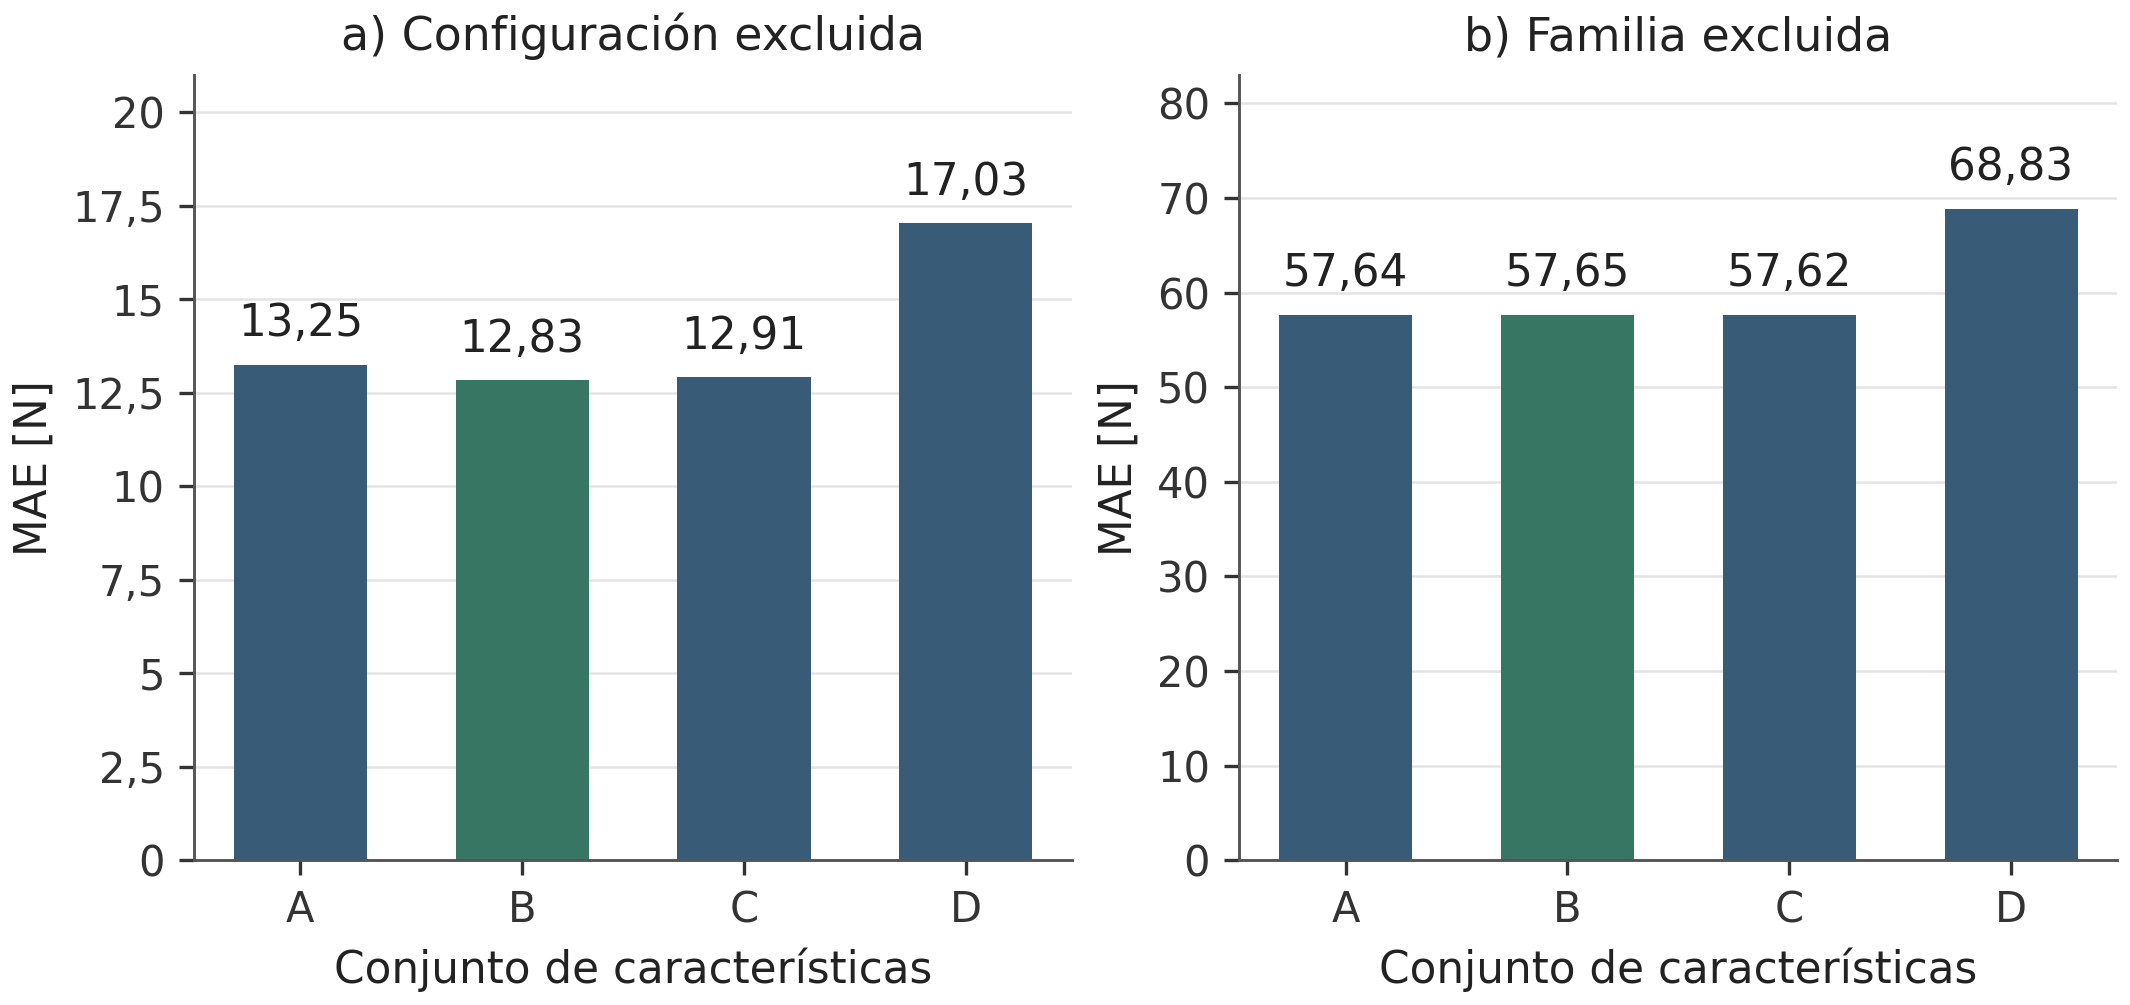
\includegraphics[width=\linewidth]{figures/01_mae.png}
\caption{MAE OOF de A--D bajo dos objetivos de generalización. La escala de cada panel se muestra explícitamente. Fuente: predicciones y métricas verificadas de la ejecución de Feature Engineering.}
\label{fig:mae}
\end{figure}

\subsection{Diagnóstico de residuales}
En B, los casos 1 y 17 fueron sobreestimados en 34,206 y 31,404~N; el caso 22 fue subestimado en 29,640~N (Figura~\ref{fig:diagnostico}). La mejora media no elimina esos errores locales. Por familia, B obtuvo MAE de 15,636, 11,853 y 11,326~N para $Y=4,5,6$. Frente a A empeoró 0,392~N en $Y=4$ y mejoró 0,653 y 0,885~N en las otras dos. No existe una mejora homogénea entre arquitecturas.

Con residuo definido como observado menos predicho, las medias fueron +4,067, $-9,832$ y +6,909~N. El patrón apunta a sobreestimación media en $Y=5$ y subestimación en las familias extremas; constituye un diagnóstico descriptivo de calibración local. Al reservar familias, los errores crecen a 52,562, 43,232 y 76,602~N. D, además, genera cuatro predicciones negativas, con mínimo de $-6,798$~N. Se conservaron sin truncar para hacer visible esa incompatibilidad con la magnitud física del objetivo.
\begin{figure}[htbp]
\centering
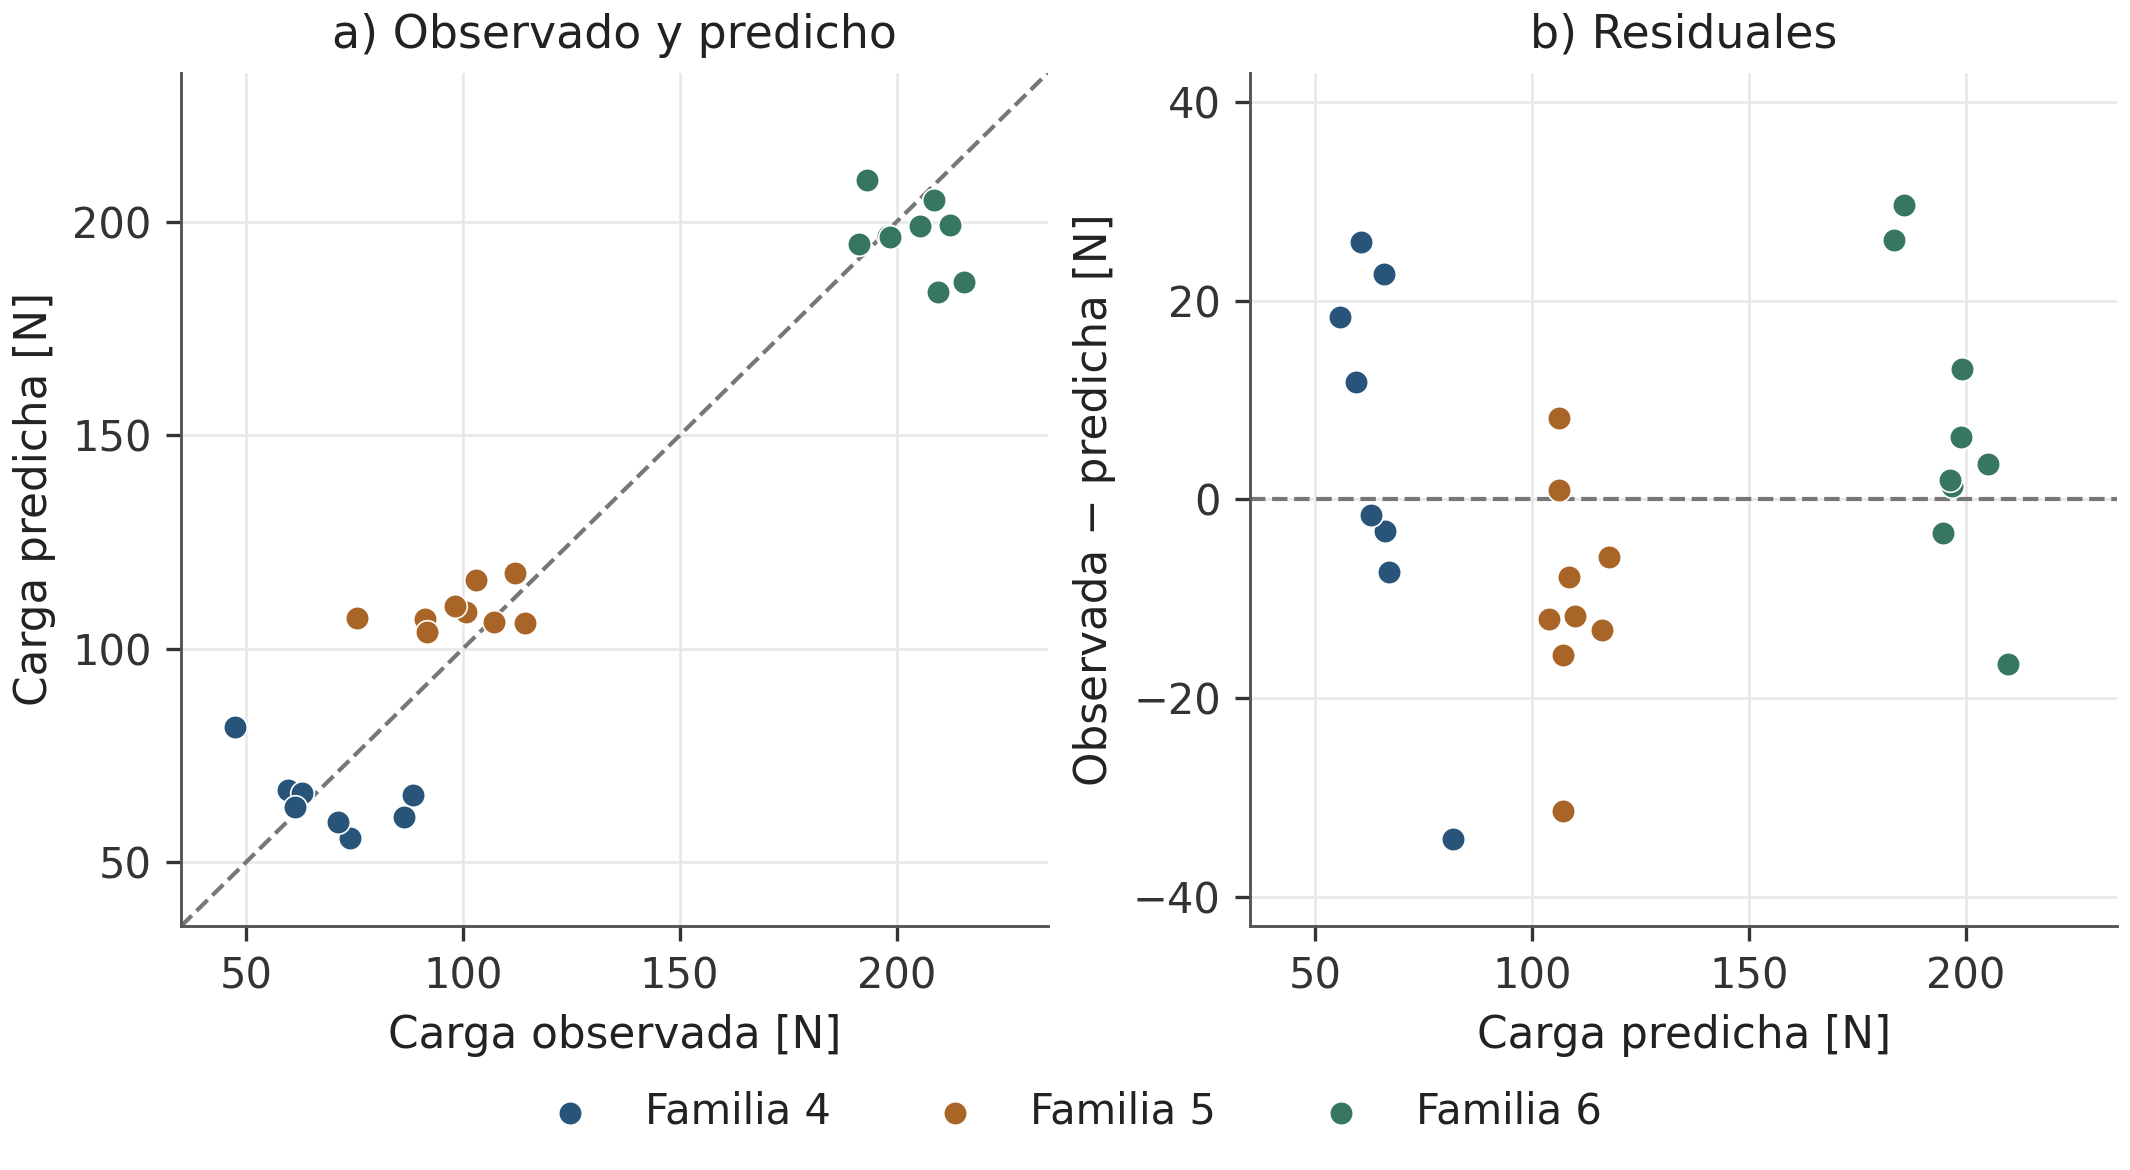
\includegraphics[width=\linewidth]{figures/02_diagnostico.png}
\caption{Predicciones OOF y residuales de B en el protocolo principal. La identidad indica predicción exacta y el cero indica ausencia de residuo. Las etiquetas identifican casos concretos; no establecen errores de medición.}
\label{fig:diagnostico}
\end{figure}

\subsection{Evaluación de estabilidad}
Para cada grupo se calculó $d_g=\mathrm{MAE}_{B,g}-\mathrm{MAE}_{A,g}$. Los contrastes varían entre $-5,423$ y +6,059~N, con mediana de $-0,312$~N (Figura~\ref{fig:pareadas}). La desviación del MAE entre folds aumenta de 9,677~N en A a 10,167~N en B: una mejora agregada puede coexistir con mayor heterogeneidad. C gana en nueve grupos respecto de B y D en siete respecto de C.

La sensibilidad disponible retira cada grupo únicamente del cálculo agregado de errores, manteniendo las predicciones ya calculadas. Bajo esa operación, $\Delta\mathrm{MAE}_{B-A}$ permanece negativo, entre $-0,671$ y $-0,211$~N. La dirección de la ventaja no depende de puntuar un solo grupo; sin embargo, la operación no reentrena los modelos y los casos retirados pudieron participar en otros ajustes. No constituye un análisis completo de influencia, un intervalo de confianza ni una prueba de superioridad estadística.
\begin{figure}[htbp]
\centering
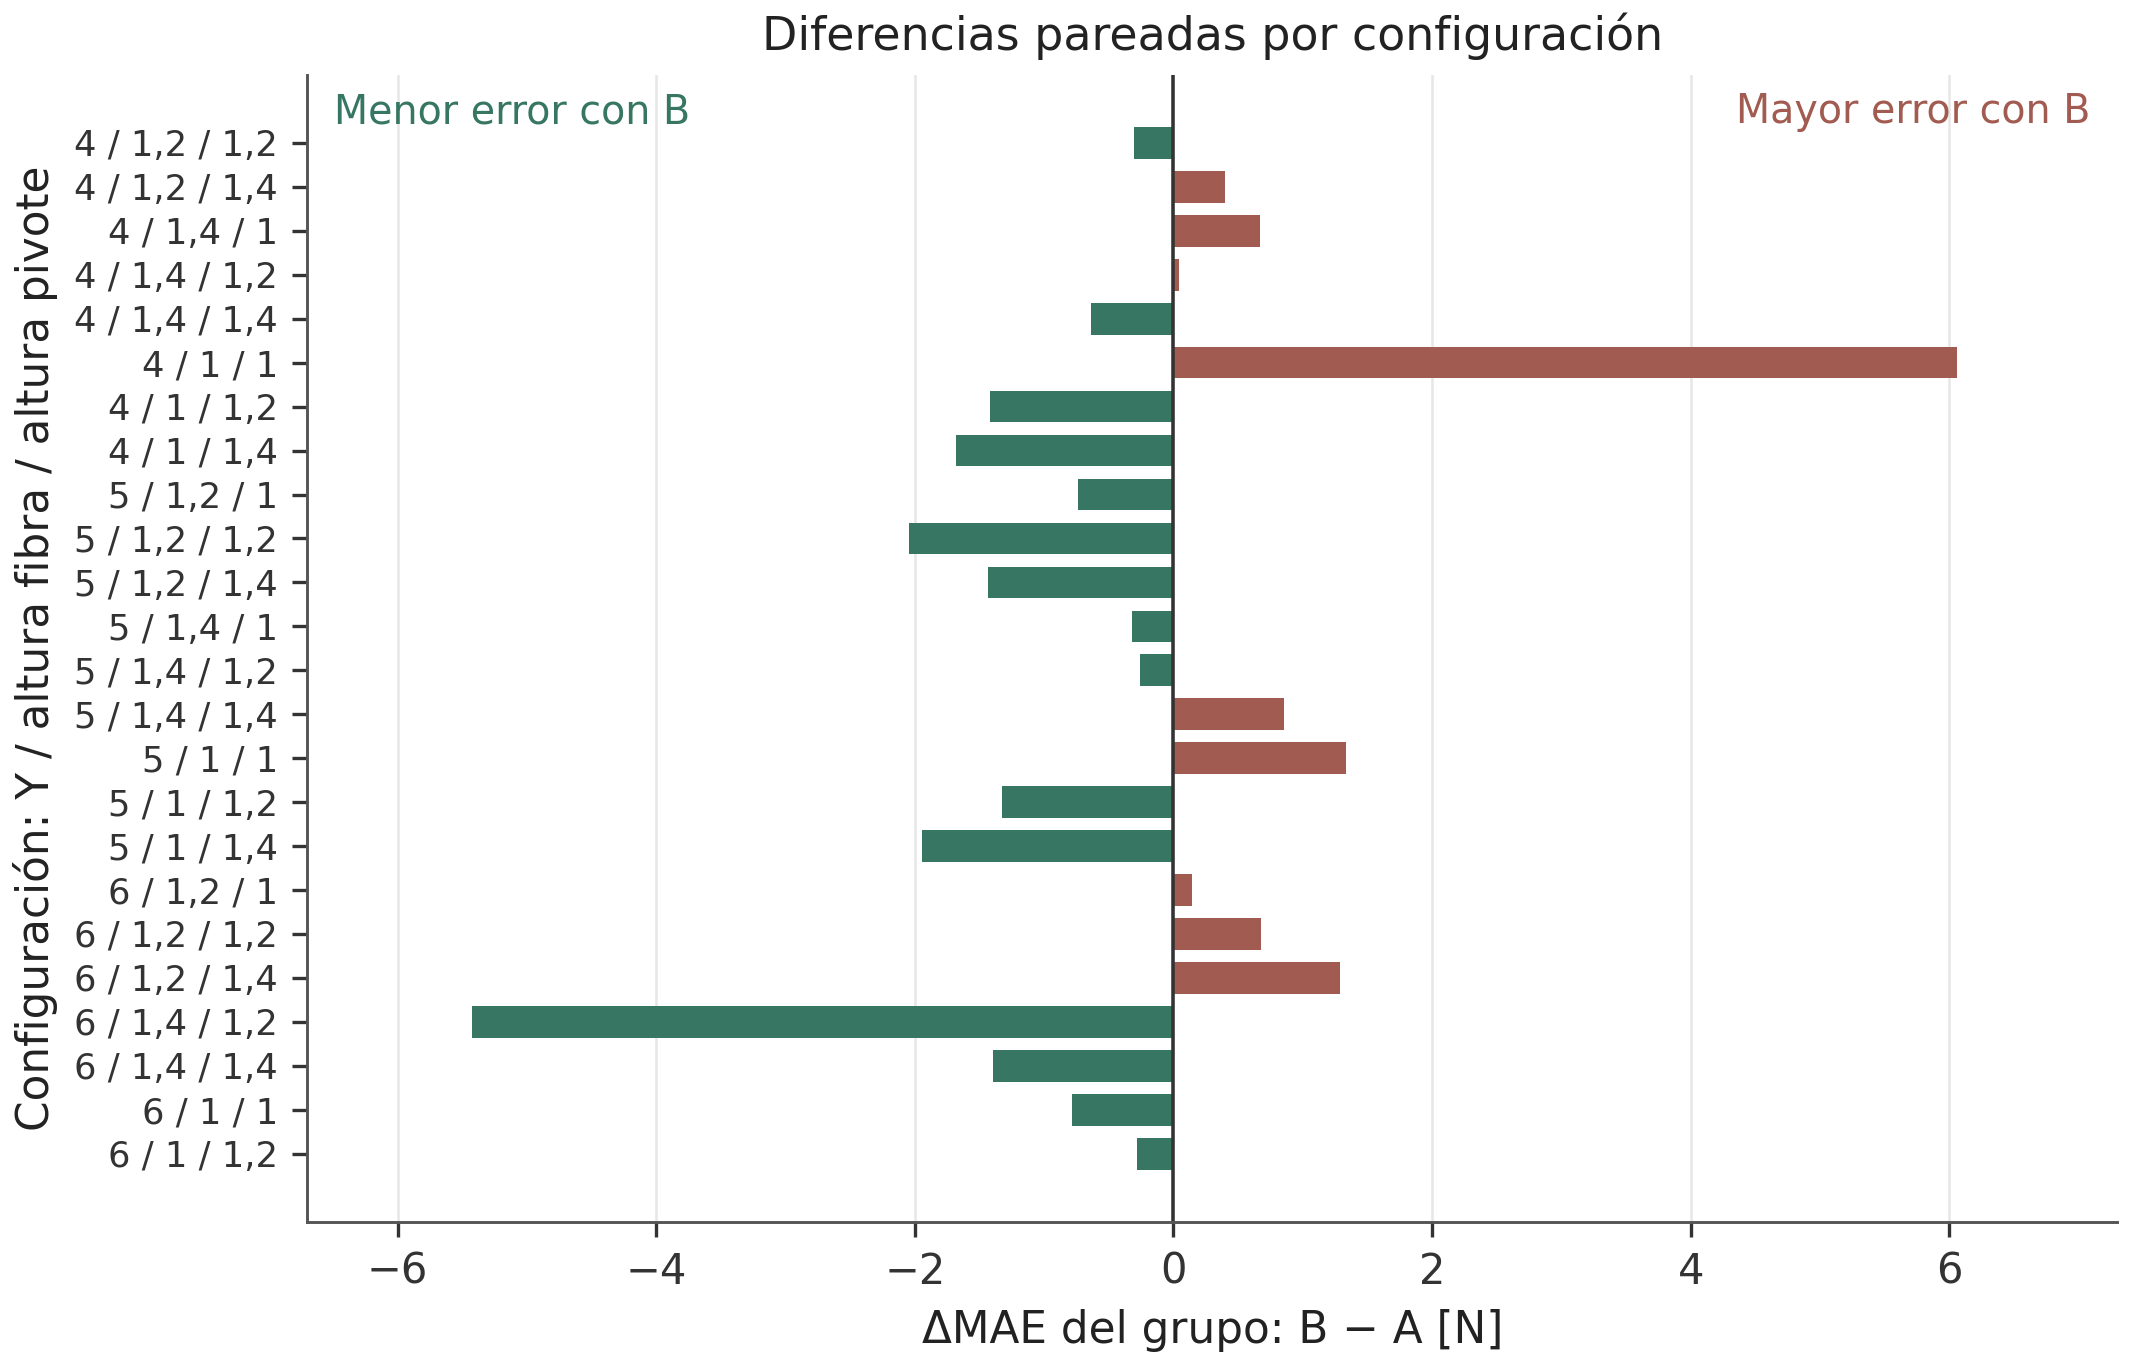
\includegraphics[width=0.94\linewidth]{figures/03_pareadas.png}
\caption{Diferencia pareada de error medio por configuración, B menos A. Valores negativos favorecen B. Cada grupo mantiene idénticos casos de evaluación entre variantes; los entrenamientos de distintos folds se solapan.}
\label{fig:pareadas}
\end{figure}

\subsection{Coste computacional}
Los tiempos de A--D fueron 0,290, 0,683, 0,571 y 0,513~s, sumados sobre los folds principales. B añadió aproximadamente 0,392~s a esa ejecución. No se registraron repeticiones de cronometraje, consumo energético ni costo monetario. Que C tarde menos que B no prueba una ventaja computacional inherente: son tiempos cortos de una sola ejecución sujetos al entorno. La decisión depende del error y de la estabilidad, no de diferencias de latencia sin un benchmark específico.

\section{Métricas e interpretación de los cinco modelos}
\label{sec:comparacion-modelos}
\subsection{Resultados con geometría original}
Los cinco regresores utilizan A, nueve características efectivas y las mismas particiones. La Tabla~\ref{tab:modelos} permite comparar funciones lineales regularizadas, modelos de similitud y conjuntos de árboles sin cambiar simultáneamente las entradas. Los parámetros son fijos; las métricas describen las configuraciones ejecutadas, no el óptimo de cada familia de algoritmos.
\begin{table}[htbp]
\centering\small\setstretch{1.0}
\caption{Cinco modelos con representación A: predicciones OOF por configuración.}
\label{tab:modelos}
\setlength{\tabcolsep}{4pt}
\begin{tabular}{@{}lrrrrr@{}}
\toprule
Modelo & MAE (N) & RMSE (N) & MedAE (N) & $R^2$ & Tiempo (s) \\
\midrule
\tableinput tablas/modelos.tex
\bottomrule
\end{tabular}
\par\smallskip\footnotesize Fuente: comparación de modelos existente. Los tiempos pertenecen a una ejecución separada de A--D; por ello el tiempo de Ridge difiere entre ambas tablas. Se suma ajuste y predicción de los folds.
\end{table}

\textbf{Ridge y bosque aleatorio.} El bosque obtiene MAE de 13,233~N frente a 13,247~N de Ridge: apenas 0,014~N menos. Su MedAE es menor (9,699 frente a 11,941~N), pero RMSE resulta casi idéntico (16,341 frente a 16,346~N). Mejora el error central sin reducir de forma apreciable el error cuadrático agregado. El tiempo observado del bosque es 4,126~s frente a 0,272~s de Ridge. La cercanía de los errores no demuestra superioridad estadística del conjunto de árboles.

\textbf{Elastic Net.} MAE de 13,979~N, 0,733~N mayor que Ridge. La combinación L1--L2 no aporta ventaja bajo esta configuración. No demuestra que deban eliminarse predictores ni que esa regularización sea inadecuada en general: se contrastaron parámetros fijos y no optimizados.

\textbf{SVR y proceso gaussiano.} MAE de 15,651 y 16,058~N, con RMSE de 19,096 y 19,341~N. Ambos superan el error de Ridge. Admitir relaciones no lineales mediante similitud geométrica no garantiza mejor desempeño. El resultado limita lo observado con estos núcleos y parámetros; no descarta otros ajustes o representaciones de esos algoritmos.

\subsection{Generalización entre familias}
\begin{table}[htbp]
\centering\small\setstretch{1.0}
\caption{Los mismos modelos y features al reservar familias completas.}
\label{tab:modelos-familias}
\setlength{\tabcolsep}{4pt}
\begin{tabular}{@{}lrrrrr@{}}
\toprule
Modelo & MAE (N) & RMSE (N) & MedAE (N) & $R^2$ & Tiempo (s) \\
\midrule
\tableinput tablas/modelos_familias.tex
\bottomrule
\end{tabular}
\end{table}
Elastic Net alcanza el menor MAE de este protocolo (57,113~N), seguido por Ridge (57,637~N); la diferencia es 0,524~N. Sin embargo, todos los $R^2$ son negativos. El bosque sube a 60,901~N y pierde su mínima ventaja del protocolo principal; SVR y proceso gaussiano llegan a 82,358 y 77,680~N. El orden de los modelos depende del objetivo de generalización, como muestra la Figura~\ref{fig:modelos}.

En el bosque, MedAE de 45,649~N coexiste con RMSE de 71,570~N: un error central menor puede ocultar errores grandes en otros casos. MAE se conserva como métrica principal; RMSE, MedAE y los errores por familia complementan su interpretación. Ninguna de estas arquitecturas resuelve por sí sola la transferencia a una familia excluida.
\begin{figure}[htbp]
\centering
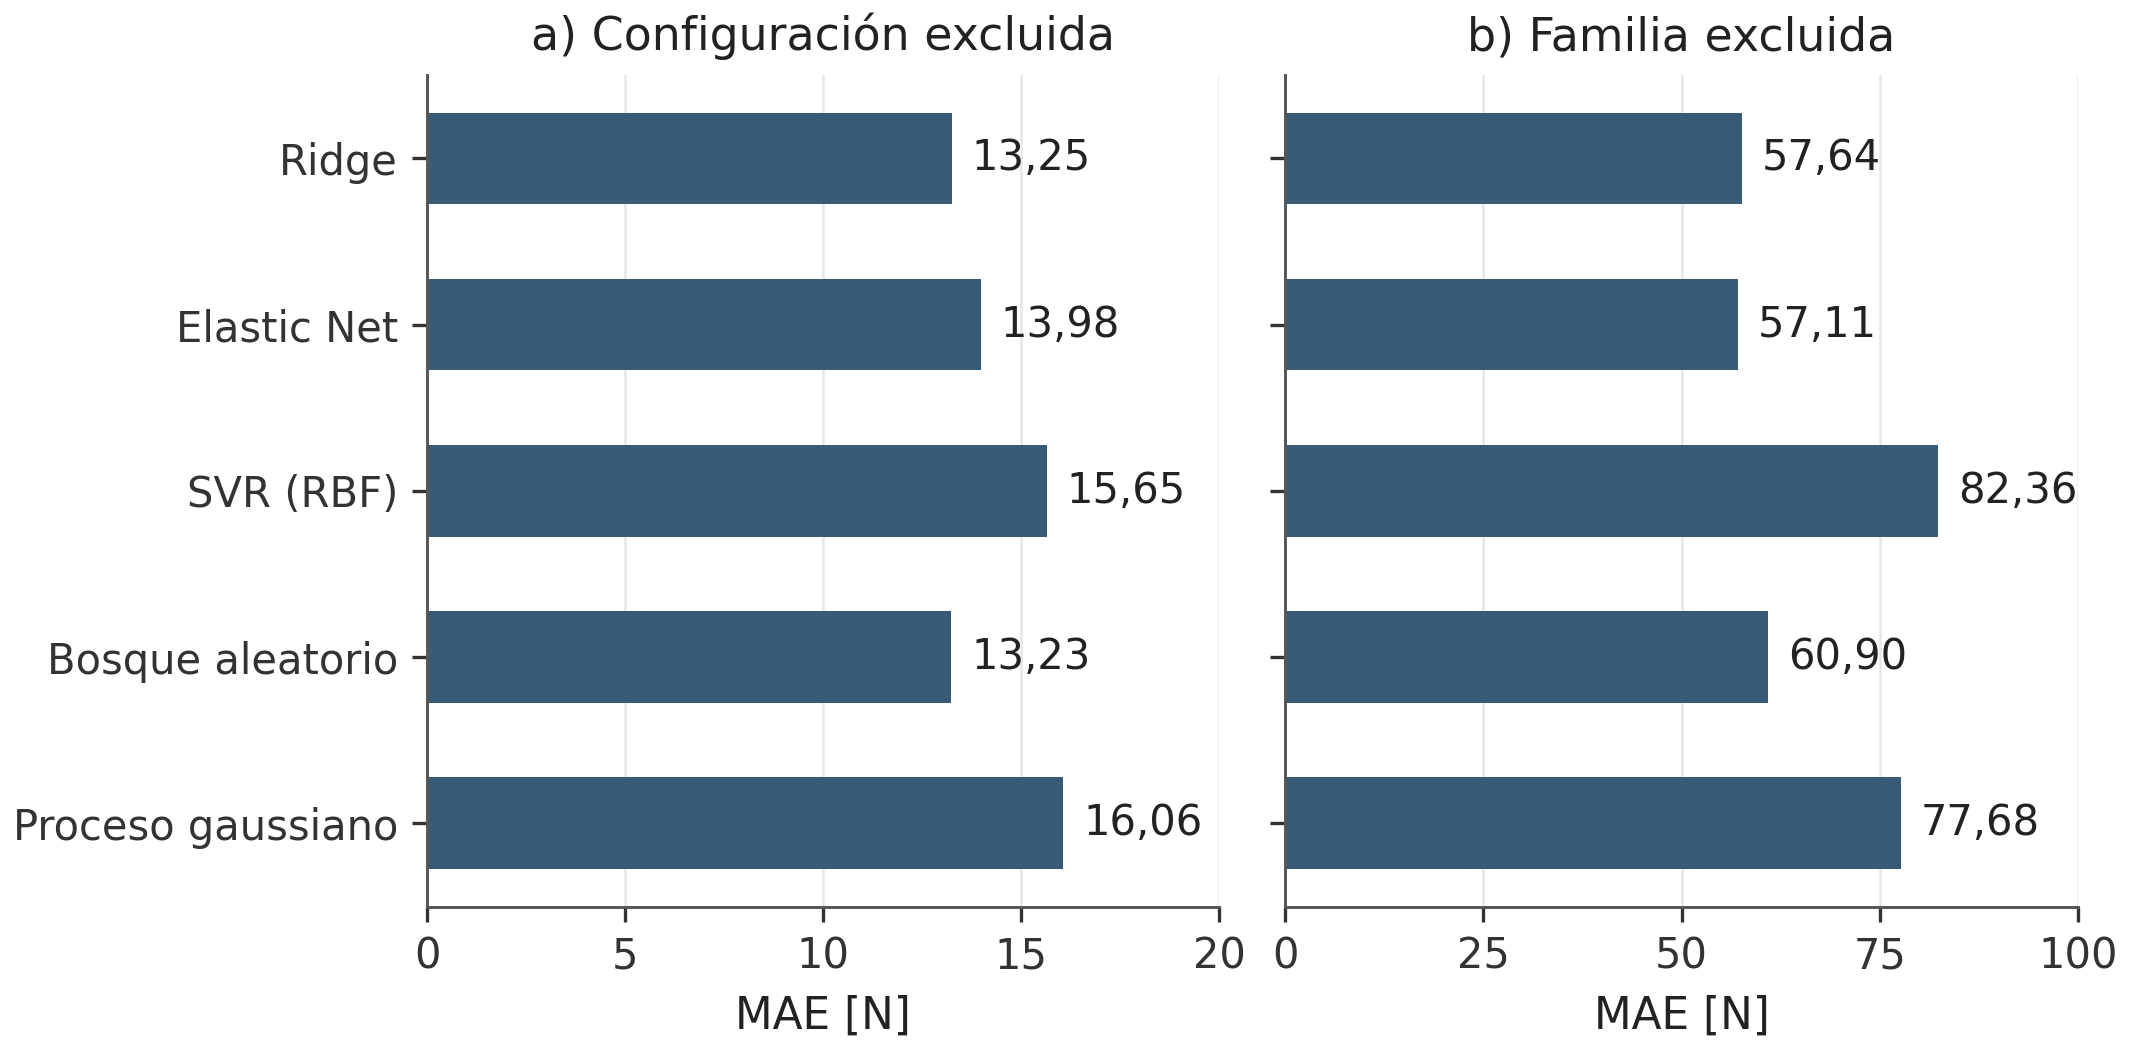
\includegraphics[width=\linewidth]{figures/05_modelos.png}
\caption{MAE de las cinco arquitecturas de regresión con geometría A. Cada panel corresponde a un protocolo y presenta su propia escala. El cambio de orden y el aumento de error obligan a distinguir configuraciones reservadas de familias completas.}
\label{fig:modelos}
\end{figure}


\section{Interpretación y decisiones del sprint}
\label{sec:discusion}
\subsection{Relación entre EDA, features y errores}
El 96,55\% de la variación del objetivo se asocia descriptivamente a diferencias entre familias. Esto ayuda a explicar el alto $R^2$ global y el deterioro al excluir una familia. La razón logarítmica presenta alta asociación global, pero no mejora B; los momentos tienen asociación condicionada cercana a cero y aportan una mejora pequeña. La correlación marginal y la utilidad para un estimador responden preguntas distintas.

Los momentos amplían la base funcional de Ridge sin añadir mediciones. Son compatibles con descripciones geométricas utilizadas en modelos que incluyen flexión \cite{turco2017,turco2019}, pero no equivalen a rigidez $EI$ medida ni identifican el mecanismo de rotura. El deterioro de D demuestra que la dependencia entre descriptores no garantiza que retirarlos conserve la predicción penalizada.

\subsection{Decisiones}
Se \textbf{mantiene A como baseline} y \textbf{B en evaluación}: su mejora de 3,11\% no cumple todos los criterios, aunque conserva dirección favorable al omitir grupos del agregado de scores. Se \textbf{descartan C respecto de B y D respecto de C}, con deterioros de 0,079 y 4,121~N. La mínima diferencia de 0,014~N entre bosque y Ridge no sustenta sustituir el algoritmo; ninguno resuelve la transferencia entre familias.

\subsection{Incertidumbre y siguiente sprint}
El procesamiento auditado se ajusta dentro de entrenamiento, pero los candidatos se propusieron usando todo el EDA, lo que mantiene sesgo de selección \cite{cawley2010}. Faltan validación externa y metadatos concluyentes de réplicas y lotes; las discrepancias de algunas geometrías también condicionan la interpretación. Los folds comparten entrenamiento y su dispersión no es un error estándar independiente.

El siguiente sprint debe congelar A y B, conciliar las discrepancias geométricas y evaluarlos sobre ensayos independientes con grupos definidos antes de observar las respuestas. Si aún no están disponibles, un análisis de influencia con reentrenamiento puede precisar la estabilidad interna; no reemplaza la validación externa. Las predicciones actuales no se proponen como límites de seguridad estructural. Las configuraciones y los comandos de reproducción se conservan en el README.
